\documentclass[crop,tikz]{standalone}% 'crop' is the default for v1.0, before it was 'preview'
%\usetikzlibrary{...}% tikz package already loaded by 'tikz' option
\begin{document}

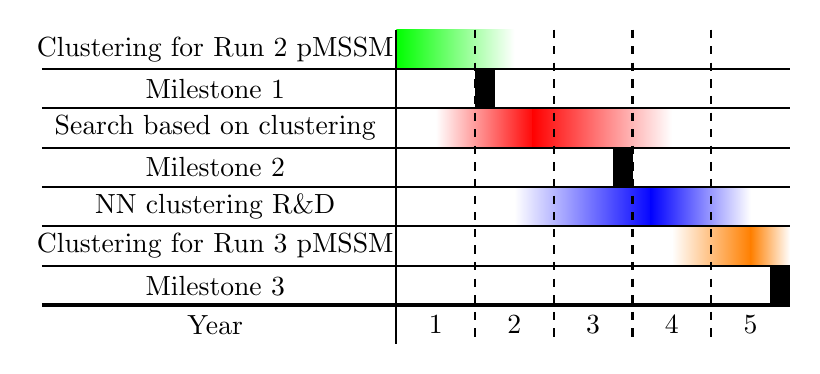
\begin{tikzpicture}[scale=.5]
  \shade[left color=green, right color=white](0,0) rectangle (3.,-1);
  \fill[color=black](2,-1) rectangle (2.5,-2);
  
    \shade[left color= white,right color=red](1,-2) rectangle (3.55,-3);
    \shade[left color=red,right color=white](3.45,-2) rectangle (7,-3);

    \fill[color=black](5.5,-3) rectangle (6,-4);

    \shade[left color=white, right color=blue](3,-4) rectangle (6.55,-5);
    \shade[left color=blue,right color=white](6.45,-4) rectangle (9,-5);
    
    \shade[left color = white, right color=orange](7.,-5) rectangle (9,-6);
    \shade[left color=orange,right color=white](9,-5) rectangle (10,-6);

    \fill[color=black](9.5,-6) rectangle (10,-7);

    \node at (-4.6,-0.5) { Clustering for Run 2 pMSSM};
    \node at (-4.6,-1.5) { Milestone 1}; % pMSSM paper
    \node at (-4.6,-2.5) { Search based on clustering};
    \node at (-4.6,-3.5) { Milestone 2}; % New search paper
    \node at (-4.6,-4.5) { NN clustering R\&D};
    \node at (-4.6,-5.5) { Clustering for Run 3 pMSSM};
    \node at (-4.6,-6.5) { Milestone 3}; % UFS+clustering paper
    \node at (-4.6,-7.5) { Year}; % UFS+clustering paper
    \node at (1,-7.5)  {1};
    \node at (3,-7.5)  {2};
    \node at (5,-7.5)  {3};
    \node at (7,-7.5)  {4};
    \node at (9,-7.5)  {5};
    
    \draw[thick](0,0) -- (0,-8);
    \draw[dashed, thick](2,0) -- (2,-8);
    \draw[dashed, thick](4,0) -- (4,-8);
    \draw[dashed, thick](6,0) -- (6,-8);
    \draw[dashed, thick](8,0) -- (8,-8);

    \draw[thick](-9,-1) -- (10,-1);
    \draw[thick](-9,-2) -- (10,-2);
    \draw[thick](-9,-3) -- (10,-3);
    \draw[thick](-9,-4) -- (10,-4);
    \draw[thick](-9,-5) -- (10,-5);
    \draw[thick](-9,-6) -- (10,-6);
    \draw[very thick](-9,-7) -- (10,-7);

\end{tikzpicture}
\end{document}